\documentclass[a4]{report}
\usepackage[utf8]{inputenc}
\usepackage[czech]{babel}
\usepackage[utf8]{inputenc}
\usepackage[utf8]{inputenc}
\usepackage[czech]{babel}
\usepackage{amsmath} 
\usepackage{amsthm}
\usepackage{amssymb}
\usepackage[acronym]{glossaries}
\usepackage{hyperref}
\usepackage{siunitx}
\usepackage{physics} % \vb bold vector http://mirrors.ibiblio.org/CTAN/macros/latex/contrib/physics/physics.pdf
\usepackage{braket}
% $\braket{\varphi|\psi}$
% $\bra{\varphi}$
% $\ket{\psi}$
% $\ket{\varphi}\bra{\psi}$
% $\ketbra{\varphi}{\psi}$
\usepackage[hscale=0.7,vscale=0.8]{geometry}
\urlstyle{same}
\usepackage{mhchem}
\def\R{\mathbb{R}}
\def\N{\mathbb{R}}


\newtheorem{theorem}{Theorem}


\newcommand{\cvec}[1]{\ensuremath{\begin{pmatrix}#1\end{pmatrix}}}

% ====================================================================
% Mathematics
% ====================================================================
\newcommand\N{\ensuremath{\mathbb{N}}}  % Set of natural numbers
\newcommand\R{\ensuremath{\mathbb{R}}}  % Set of real numbers
\newcommand\Z{\ensuremath{\mathbb{Z}}}  % Set of integer numbers
\renewcommand\O{\ensuremath{\emptyset}} % Empty set
\newcommand\Q{\ensuremath{\mathbb{Q}}}  % Set of rational numbers
\newcommand\C{\ensuremath{\mathbb{C}}}  % Set of Complex numbers
% Exponenciel function
\newcommand{\e}[1]{\ensuremath{ {\rm e}^{#1} }}

\theoremstyle{definition}
\newtheorem{definition}{Definition}[section]

% ====================================================================
% Physics
% ====================================================================

% Continuum Mechanics
\newcommand\Stress{\ensuremath{\mathbf{\sigma}}} % stress
\newcommand\Strain{\ensuremath{\mathbf{\epsilon}}} % strain

%Numbered environment
\newcounter{example}[section]
\newenvironment{example}[1][]{\refstepcounter{example}\par\medskip
   \noindent \textbf{Example~\theexample. #1} \rmfamily}{\medskip}



\title{
%MATEMATICKÉ A NUMERICKÉ MODELOVÁNÍ, STATISTIKA, FYZIKA \\ 
STUDIJNÍ POZNÁMKY
}

\begin{document}
    \maketitle
    % \tableofcontents

    % % Mechanika a termodynamika kontinua a teorie směsí.
\part{Mechanika kontinua}

Poznámky ze vychází s přednášek M.L, O.Č a skript Málek a Souček 2021.

\section{Zápisky ze schůzek}

\begin{enumerate}
    \item Probrat kapitolu 1 Callen 
\end{enumerate}


\chapter{Matematický aparát}

\section{Matice}

\begin{enumerate}
    \item transpozice, inverze: $(A \cdot B)^T = B^T \cdot \A^T, \quad (A \cdot B)^{-1} = B^{-1} \cdot A^{-1}, \quad (A^{-1})^T = (A^T)^{-1}$
    \item ortogonální matice:  $Q^T = Q^{-1}, \quad Q^T \cdot Q = Q \cdot Q^T = I, \quad |Det(Q)| = 1 $
    \item vlastní čísla  vektory: $A \cdot \vb v = \lambda \vb v$
    \item determinant $Det(A \cdot B) = Det(A) \cdot Det(V) $
    \item Diagonalizace matice
    \item Pozitivní definitnost matice
    \item Mocnina respektive odmocnina matice
    \item $T : U$ kontrakce tenzorů
\end{enumerate}

\section{Vektory}
\section{Tenzory}

tenzor prvního řádu, tenzor druhého řádu, tenzor třetího řádu, Levi-Civitův tenzor $\epsilon_{ijk}$, 

\subsection{Operátory}

Jakobián a diferenciální operatory: grad, curl (rot), div

\chapter{Kinematika}

Kinematika neboli studium pohybu.

V mechanice kontinua si pohyb tělesa $\mathfrak{B}$ představujeme jako funkci $\chi = \chi(\vb X, t)$, která zobrazuje jeho počáteční polohu $\vb X$ do konečné polohy $\vb x = \chi(\vb X, t)$.

Pomocí velkého písmene označujeme referenční konfiguraci např. $\vb X$ a pomocí malého písmene označujeme aktuální konfiguraci např. $\vb x$.

\begin{equation}
    \chi(\dot, t) : \kappa_0(\mathfrak{B}) \to \kappa_t(\mathfrak{B}) 
\end{equation}

Prostorový gradient:

\begin{gather}
    Grad[\Phi(\vb X, t)] = \pdv{\Phi}{\vb X} \\
\end{gather}

\chapter{Deformace}

\subsection{Předpoklad kontinuity}

Předpokládáme, že funkce $\chi, \ldots$ jsou dostatečně pekné a hladké: jednoznačné, invertovatelné, derivovatelné do libovolného rádu až na vybrané singulární body, křivky, povrchy. Zaručujeme si tím, že těleso má konečný objem tzn. nemůžeme ho deformovat tak, že bude mít nulový nebo nekonečný objem a dále, že těleso zachovává dimenzionalitu tj. objem se deformuje na objem, povrch na plocha na plochu (povrch) a křivka na křivku. Při tomto předpokladu tedy nelze uvažovat o vzniku nových povrchů, lomu, trhhlinách a jiných diskontinuitách.


\subsection{Materiálový popis}
\subsection{Referenční popis Lagrangeův}
\subsection{Prostorový popis Eulerův}
\subsection{Relativní popis}

\subsection{Materiálový popis}
\subsection{Referenční popis Lagrangeův}
\subsection{Prostorový popis Eulerův}
\subsection{Relativní popis}


Polární rozklad deformačního gradientu je analogiií rokladu komplexního čísla na $r$ a $\phi$ např. $z = Re + Im = x + iy = r \exp(i\phi)$, kde $r = \sqrt(x^2 + y^2)$ a $\phhi = \atan(\frac{y}{x})$.

Tenzor s nenulovým determinatem můžeme rozložit na orotogonální tj. rotační složku (tenzor) a levý nebo pravý \textit{stetch} symetrický  a pozitivně definitní tenzor.

$$
    F = R \cdit U = V \cdot R
$$

Green, Piola, Finger, Cauchy deformační tenzor.


    \part{Termodynamika a statistická fyzika}

Zde vnzikající text  slouží jako poznámky k předmětu Teorie tekutin a směsí a pokrývají základy termodynamiky a statistické fyziky, nutné pro pochopení látky, ale značně ji přesahují. Proto snad budou použitelné obecně, jako základní přehled tohoto tématu. Následuje seznam otázek, termínů (hesel), která je třeba definovat, vysvětlit a zasadit do kontextu.

\begin{enumerate}
    \item termodynamický děj
    \item termodynamický proces
\end{enumerate}

\begin{thebibliography}{}
\bibitem{Callen1985} Callen, 1985
\end{thebibliography}

\chapter{Rovnovážná termodynamika}

\section{Makroskopická vs mikroskopické pozorování}

Makroskopický popis určuje vlastnosti systému z makroskopicky měřitelných veličin.

Statisticý popis..

Přenost tepla, probíhá okamžitě, např. při zahřátí tělesa, tj. dodání tepla, se toto projeví v celém objemu tělesa najednou. V klasické rovnovážné termodynamice zanendbáváme čas a tudíž změna působí na systém okamžitě.

Rovnovážná termodynamika \textit{equlibrium thermodynamics} se zabývá vratnými procesy, proto také někdy mluvíme o vratných termodynamických procesech a vratně termodynamice (\textit{reversible}).

V této kapitole zavedeme klasicky (fenomenologicky) základní principy, postuláty a zákony na kterých stojí rovnovážná termodynamika. Způsob, jakým byly tyto zákonitosti objevovány a jak jsou popsány v učebnicích je velmi různorodý. Myslím, že pro důkladné pochopení se vyplatí podívat se do vícero zdrojů, které na problém hledí z různých hledisek. Pro začátek doporučím knihy \cite{Callen1985}.

\section{Systém, hranice a okolí}

Jako \term{systém} $\mathfrac{S}$ označíme oblast $\Omega$ prostoru ($E^3$), oddělený od \term{okolí} skutečnou nebo myšlenou hranicí $\partial \Omega$, jehož vlastnosti chceme popisovat. Podle vlastností hranice rozlišujeme následující druhy systému.

\begin{enumerate}
    \item \textbf{Otevřený} systém může vyměňovat s okolím energii a hmotu.
    \item \textbf{Uzavřený} systém  může vyměňovat s okolím pouze energii.
    \item \textbf{Izolovaný} systém nemůže vyměňuje s okolím hmotu ani energii.
\end{enumerate}

Uvedená hranice systému se také označuje jako stěna (\textit{wall}). Jkao skutečnou hranici si můžeme představit nádobu. Jako myšlenou hranici např. povrch krystalu v tavenině,

Stěna může být 
\begin{enumerate}
    \item \textbf{Adiabatická} stěna
    \item \textbf{Diatermická} stěna
\end{enumerate}


\section{Stav termodynamické rovnováhy systému} 

Rovnovážná termodynamika popisuje stavy systému, ve kterých se makroskopicky pozorovatelné veličiny v čase (zdánlivě) nemění a jsou tak rovny časově středním hodnotám. Makroskopický systém je ve stavu termodynamické rovnováhy, pokud se žádné makroskopicky pozorovatelné (pozorované) veličiny v čase nemění. Mluvíme o kvazistatických procesech, kdy systém přechází z jednoho rovnovážného stavu do dalšího  a tím se mže dostat daleko od původního stavu skrze sekvenci rovnovážných stavů jen malou změnou podmínek.

\textbf{Postulujeme}, že každý izolovaný systém dospěje při $t \to \infty$ do stavu rovnováhy, tj. stav, ve kterém se již jeho makroskopické vlastnosti v čase nemění. tento stav je určen pouze vnitřními faktory a nikoliv např. dříve působícími vnějšími vlivy (silami). Systém ve stavu termodynamické rovnováhy není závislý na předchozích stavech tj. na historii. Např. pokud vhodíme kostku ledu do sklenice a necháme ji v místnosti dostatečně dlouho, tak led roztaje a systém se dostane do rovnováhy s okolím. V tomto stavu nejsme schopni rozpoznat z jakého stavu do rovnováhy systém došel. Bylo to tání ledové kostky nebo prosté přilití vody do sklenice? Obecně mají fyzikální systémy paměť, kdy jejich vývoj je odezvou na předchozí stav systému a interakci s okolím. $\imply$ vývoj systému je nevratný na rozdíl od systému bez paměti.  Systémy jsou symetrické vzhledem k otočení šipky času.

\subsection{Popis rovnovážného stavu pomocí makroskopicky měřitelných veličin}

závislé a nezávislé stavové veličiny, stavová rovnice

\section{Teplota, energie a entropie}

\section{Postuláty klasické termodynamiky}

Jako jednoduchý systém označíme takový, který je popsatelný několik málo makroskopicky měřitelnými parametry jako je tlak, objem, teplota.  

\begin{theorem}
Pro jednoduchý systém existuje stav nazývaný rovnovážný stav takový, že ho lze, z makroskopického pohledu, popsat vnitřní energií $U$, objemem $V$ a molárním množstvím $N = \sum N_i$ jeho chemických komponent.  
\end{theorem}

Dále uvedeme postuláty o maximu entropie.

\begin{theorem}
Pro každý rovnovážný stav existuje funkce extenzivních parametrů nazývaná entropie $S$ taková, že \ldots 
\end{theorem}

Pokud známe entropii systému jako funkci extenzivních parametrů, pak všechny jeho termodynamické vlastnosti z ní můžeme odvodit. Proto tomuto vztahu říkáme \textit{fundamentální vztah}.

\textbf{Entropie je zavedena pouze pro rovnovážný stav!}

Tato formulace postulátů je převzata z \cite{Callen1985}.

\section{Zákony klasické termodynamiky}

Klasická termodynamika zavádí (postuluje) tzv. termodynamické zákony (též postuláty) které považujeme za platné a souhlasící s experimentem. Někdy jsou též nazývané \textit{větami}, což by ale naznačovalo, že je lze nějak dokázat, proto je budeme nazývat zákony nebo též postuláty. Známe tzv. tři termodynamické zákony, ale předchází dodatečně formulovaný nultý zákon, o kterém je také dobré něco vědět. 

\subsection{0. termodynamický zákon}

(\textit{zero law of thermodynamics})
    
\subsection{1. termodynamický zákon}

(\textit{first law of thermodynamics})

\subsection{2. termodynamický zákon}

(\textit{second law of thermodynamics})

\subsection{3. termodynamický zákon}

(\textit{third law of thermodynamics})

0. termodynamický zákon: existence empirické teploty jako intenzivní veličiny

1. termodynamický zákon: existence vnitřní energie 

$$
    U = Q + W 
    dU = \delta Q + \delta W
$$

Pod symbolem práce se skrývají různé formy např. mechanická, chemická, elektromagnetická.

2. termodynamický zákon: existence entropie $S$
3. termodynamický zákon: $\lim_{T \to 0} S = 0$

\section{Termodynamický proces a rovnováha}

\section{Fyzický model systému v termální rovnováze}

Poznámky k [Málek a Souček, 2020]

Teorie interakcí v kontinuu se dá rozdělit na dva přístupy

1. všechny komponenty směsi spolu koexistují [Truesdell, Toupin] viz \textit{continuum mixture theory}
2. [Drew Passman] \textit{multi phase theory}
    Jak to souvisí s phase-field metodou (otherwise called diffuse interface)

\begin{itemize}

\item \textbf{Princip minimalizace energie $E$} -- rovnovážná hodnota nijak neomezeného vnitřního parametru je taková, že \textit{minimalizuje vnitřní energii} pro danou celkovou entropii.

\item \textbf{Princip maximalizace entropie $S$} -- rovnovážná hodnota nijak neomezeného vnitřního parametru je taková, že \textit{maximalizuje entropii} při dané celkové vnitřní energii.

\end{itemize}

\subsection{Konkavita entropie $S$}

\subsection{Konvexita energie $E$}

\subsection{Entropie při složení dvou systémů}

$$
S^C = S^{A + B} = S^A + S^B 
$$

\section{Jednosložková jednoduchá tekutina}
jednosložková neboli jednokomponentní

NVE

Jak se zvýší entropii jednosložkového systému?

\section{Vícesložková jednoduchá tekutina}
vícesložková neboli vícekomponentní uniformní složená z komponent

E

\section{Extenzivní parametr}

\section{Intenzivní parametr}


\textbf{Entropie a Energie nejsou přímo měřitelné, zatímco T, P, V ano.}


% \subsection{van der Waals Equation}

% Calculate the constants (parametres) $a$ and $b$ for $\ce{H2O}$ in the van der Waals and in the Redlich-Kwong equations. 

% Vezmeme kritické hodnoty z tabulek a pozor na jednotky R.

% \begin{equation}
% \left( P + \frac{n^2a}{V^2} \right) \left( V - nb \right) = nRT
% \end{equation}

% For 1 mole the equation simplifies to 

% \begin{equation}
% \left( P + \frac{a}{V_m^2} \right) \left( V_m - b \right) = RT
% \end{equation}

% % http://www2.ucdsb.on.ca/tiss/stretton/database/van_der_waals_constants.html
% % The constants a and b are called  van der Waals constants. They have positive values and are characteristic of the individual gas. If a gas behaves ideally, both a and b are zero, and van der Waals equations approaches the ideal gas law PV=nRT. 
% % a = 5.537 -- provides a correction for the intermolecular forces.
% % b = 0.03049 --adjusts for the volume occupied by the gas particles.

% \subsection{Redlich-Kwong Equation}

% \section{Two Point Eutectic System}
    
% \subsection{Congruent Melting and Eutectic Point}

% \chapter{Příklady z klasické chemické termodynamiky}

% Uvažujem stále množství ideálního plynu při výchozí teplotě \SI{20}{\celsius}


% % Let $S$ be an isolated thermodynamical system with constatnt energy E (U?), consisting of $N$ particles, where N is a sufficiently large number, so that it is not possible to know the energy of a individual particle. 

% % We can only know the  
% % \subsection{Helmholz Free Energy}
% % \subsection{Gibbs Free Energy}
% % \begin{equation}
% %     G = H -TS    
% % \end{equation}

% % \begin{equation}
% %     dG = dH - sdT - TdS
% % \end{equation}

% % Gibbs free energy is a thermodynamic potential that can be used to calculate the maximum reversible work that may be performed by a thermodynamic system at a constant temperature and pressure.

\section{Maxwellovy rovnice}

\section{Gibbsovy-Helmholtzovy rovnice}

\chapter{Statistická termodynamika}

% \subsection{Boltzmann Distribution}

\chapter{Kinetická teorie plynu}

\section{Model ideální plynu}
\subsection{}

Mějme plyn skládající se z jednoho druhu hmotných částic o stejné hmotnosti $m$, které spolu neinteragují jinak než pružnou srážkou tzn. že při srážce se jen změní směr rychlosti částice. Částice mají stejnou rychlost.
Entropie izotermální expanze ideálního plynu.
Entropie izotermální komprese ideálního plynu.


Otázky pro B. Gaše: Dobrý den, 

První termodynamický zákon se uvádí v podobě $ U = Q + W $, nebo diferenciálně $ dU = dQ + dW $, kde $Q$ značí teplo a $W$ práci. V různých učebnicích ale různě uvádí,  co vše se zahrnuje pod $W$, např., 
mechaniská, elektrická, magnetická, chemická. Jaké všechny členy tedy pod $W$ zahrnout, pokud by měl výčet být úplný?

Na ideální plyn klademe tyto předpoklady:

\begin{itemize}
    \item 
\end{itemize}

\chapter{Nerovnovážná termodynamika}


    
    % 
\section{Atom}

\subsection{Bohrův model atomu}

\subsection{Magnetické vlastnosti}
Zeemanův jev


\section{Molekula}

\subsection{Symetrie molekuly}

\subsection{Pohyb a energie molekuly}

Pro dvouatomovou molekulu můžeme uvažovat vibrační , rotační  a translační pohyb.

Pro vibrační pohyb lze pracovat s Lenard-Jonesovým, Morseovým nebo parabolickým (harmonickým) potenciálem.


Pro vibrační pohyb dvoutaomové molekulu můžeme použít 
Pro rotační pohyb můžeme uvažovat 1) tuhý rotátor tzn. rychlost rotace nemá vliv na vzdálenost mezi atomy.
To platí jen do určité míry, ale pro nízké 

\subsection{Měrné teplo}

Debeyův a Einsteinův model

Pokud roztočím molekulu, můžu pozorovat i vibrace tzn rotačně vibrační stavy. Tyto stavy jsou kvantovány. Pokud na ni posvítím, můžu pozorovat absobční nebo při chlazení emisní rotačně-vibrační spektra.

\subsection{Elektronová struktura molekul, vazby, LCAO}

Co drží molekulu pohromadě? Zřejmě interakce elektronů mezi sebou a jaké vazby mezi sebou vytvářejí.

Vazby známe kovalentní při které dochází ke sdílení elektronů (překryv hustot elektronů), iontová vazba funguje jako předání elektronu mezi atomy, kdy vzniknou opačně nabyté ionty, které se přitahují např. při interakci \ce{Na} a \ce{Cl} $\imply$ \ce{Na+} a \ce{Cl+}
S kovalentní vazbou je spojena elektronegativita, s iontovou vazbou zase afinita a excitace. 

Pokus o vysvětlění vodíkové vazby Heitler a London (1927).
Magnetické vlastnosti \ce{N2} a \ce{O2} se liší! nenulová magnetická složka spinu indukuje magnetismus viz kyslík.

Pauliho vylučovací princip  Hundova [:Handova:] pravidla.

Linera Combination of Atomic Orbitals (LCAO) aproximace. Ve výchozím stavu máme dva vodíkové atomy daleko od sebe a poté je přibližujeme.
Hledáme elektonovou strukturu molekuly $H2+$.


Hybridizace a překryv orbitalů. Uhlík a hybridizace a tvorba čtyřvazných molekul

Bor...
    
    % \chapter{Kvantová mechanika (nerelativistiská)}

Pravděposobnostní popis, komutátor, operátor, operátor pozice, operátor hybnosti,  relace neurčitosti, Schrodingerovat rovnice bezčasová 

\section{Příklady k přednáškám }

Poruchový počet


\section{Vodíku podobný atom}
\label{QM.30.01.2021}

Uvažujeme jeden elektron a jádro sestávající z 1 až Z protonů.
Podle klasické fyziky by atom vodíku neměl být vůbec stabilní

Hamiltonián

$$
    H = -\frac{h^2}{2} ...
$$

Jádro berem jako nekonečně těžké


pro konečné hmotnosti jádra


pro limitu $r \to \infty$ je Coulombův potenciál do nuly


Vlnová funkce bude záviset na kvantových číslech z momentu hybnosti
a dodatečné hlavní kvantové číslo $n$


$$
    \psi = \psi_{nlm}(r, \Phi, \phi)
$$


integrály pohybu znamená že se zachovává energi


Řešení Shcrodingerovy rovnice pro atom vodíku

$$

    \hat{H} = \frac{h}{2m} ...
$$


$$
    \hat{L}^2 = -h^2\Delta_{\Phi, \phi}, \quad \hat{L}_z = -ih prt[Phi]
$$


Vlnová funkce pak bude mít tvar


Využijeme substituci

$$
	R(r) = \frac{u(r)}{r} \therefore \ldots
$$

Pro jednoznačnost přejdeme k bezrozměrných jednotek

Zde $a$ je bohrův poloměr

$$
    a = 4\pi\epsilon_0 \frac{h}{me^2}
$$

Také zavedeme berzoměrnou energii


Požadujeme aby vlnová funkce byla normalizovaná
$$
	\int_{0}^{\infty} {|R(r)|}^2 r^2 dr = 1
$$$$
    \eta = \frac{}
$$
Vnejniřším řádu to vede na podmínku $\gamma (\gamma - 1) =  l(l + 1)$

Tím pádem máme dvě možné hodnoty: $\gamma = l + 1$ a \gamma = -l$


Pro tu druhou ale $\rho \to  \infty$ diverguje.

Dosadíme do $f(\rho)$  do rovnice (řady) $\frac{d^2}{d\rho^2} - 2\alpha \ldots$

Má platit pro libovolné $\rho$

pro koeficienty tak musí platit rekurentní vzorec
$$
	a_{\nu + 1} = \frac{2\alpha (\nu + l + 1) - 2Z}{(\nu + l + 2)(\nu + l + 1)-l(l + 1)} a_{\nu}, \quad \nu = 0, 1, \ldots
$$Jak se řada chová pro velmi vysoké indexy?
Pokdu $\nu$ bude dost velké pak bude dominovat a vede to na rozvoj exponenciely.
taková nekonečná řada se dá sečíts a vyjde $f = \rho^{l + 1} e^{2\alpha\rho}$, potom by ale vlnová funkce v limitě $\rho \to \infty$ divergovala a  tedy místo nekonečné řady musíme mít polynom konečného řádu a dostaneme konečnou řadu. Musíme tedy řadu zastavit na konečném indexu $\nu$. Pro jsitou hodnotu $\nu = n_r$ musí být nulový čitatel.
Z toho plyne $2\alpha(n_r + l + 1) = 2Z, \quad n_r = 0, 1, \ldots$

Toto je kvantovací podmínka pro $\alpha = \sqrt{-\epsilon}$

pro bezrozměrnou energii pak dostaneme

$$	
	\epsilon = -\alpha^2 = - \frac{Z^2}{n^2}, \quad n = 1, 2, \ldots
$$Energie vodíku pak vyjde v základním stavu

$$
	E_n = - \frac{1}{4\pi\epsilon_0}  \frac{Z^2e^2}{}
$$Energie $E_n$ v Couloumbickém potenciálu jsou

[obr]

Energie základního stavu není degenerovaná avšak energie všech excitovaných stavů jsou degenerované a ta je rovna $\sum_{l=0}^{} (2l + 1) = n^2$

Celkovou vlnovou funkci poté dostaneme dosazením ... do $f(\rho)$


\subsubsection{Laguerrovy polynom}

Vlnové funkce několika nějnižších stavů jsou
$$
R_{n=1,l=0}(r) = \frac{Z}{}  
$$Pravděpodobnost nalezení elektrony v daném objemovém elementu zadaném $(r, r + dr)$, $\theta, \theta + d\theta)$, $(\varphi, \varphi + d\varphi)$.

Integrací přes prostorový úhel dostaneme pak...

radiální hustoty pravděpodobností $P_{nl}(r) = |R_{nl}|^2r^2$.

S rostoucí energií se pravděpodobnost nalezení elektronu vzdaluje od jádra.

s, p, d stavy

Polární diagram ukazují závislost 


Při přechodu z jednoho stavu do druhého se musí vyzářit jeden foton. Můžeme přecházet diskrítně mezi hladinami a pro každý přechod se přísluší jeden foton.

fe+25, kde se vyskytuje
přechod od rel k nerel?
kvantová elektrodynamika

\section{Spojité spektrum}

\chapter{Metoda Free Electron Molecular Orbita (FEMO)}
\label{QM.07.05.2021}

Ve složitějších látkách neumíme přesně řešit (určit) Schrödingerovu rovnici 
Při předpokladu ,že můžeme zanedbat vliv interakce elektronů, pak můžeme použít metodu FEMO.

Aplikace na $\pi$ elektrony v $1,3$ butadienu.

Máme čtyři elektrony (fermiony), každý y nich může mít spin $\pm \frac{1}{2}$.

Slaterův determinant umožňuje generovat bázové funkce.

Funkce jsou ortonormální.

Vlnové funkce budou kombinacemi funkcí $\psi_1$ a $\psi_2$

Vlnová funkce musáí být anti

Pro efektivní šířku potenciálové jámy použijeme hodnotu $L = 4 \times 1.4 \time 10^{-10} \SI{m}$.

Pro vlnovou délku fotonu 


Pro složitější molekulu např. $1, 3, 5$ \ldots


\subsection{Molekula benzenu}
Metodu FEMO můžeme použít i pro uzavřenou molekulu jako je cyklická, kruhová molekula benzenu.
Benzen má $3$ dvojné vazby a $6-\pi$elektronů

Máme dvě rovnice $ A ¤\sin 0 B \cos 0 = A \sin kL +  \cos KL $ a další rovnice plyne z podmínky spojitosti derivace $ D_t \psi(0) = D_t \psi(L)$

$$
A k  \cos(0) - Bk\sin0 \ldots
$$

a dostaneme maticovou soustavu, pro kterou determinant musí být nula, abychom měli netriviální řešení

To vede na rovnici $\cos kL = 1$ a získáme podmínky 

$$
kL = 2n\pi\ quad n = 0, \pm 1, \pm 2, \ldots
$$

Energie bude 

$$
E_n = {(2n)^2 h^2}{8mL^2}
$$

Jaké jsou vlnové funkce?

$$
\begin{gather}
    \psi_0 = \sqrt{\frac{1}{L}}    
\end{gather}
$$

    % \chapter{Fonony}

Mějme lineární řetěz stejných polarizovatelných molekul $A_1A_2A \cdots A_n$. Molekuly jsou fixované na svých pozicích.
Systém je při nulové teplotě, proto v mříži nebudou přítomny akustické fonony. Určte disperzní křivku  $\omega(k)$ a 
diskutuje chování $\omega(0)$ pro různé hodnoty $\alpha$. Pro molekulu $n$ máme zadánu pohybovou rovnici

\begin{equation} \label{Eq.phonons}
    \pdv[2]{p}{t} = -\omega_0^2 p + E \alpha \omega_0^2
\end{equation}

Rovnice \ref{Eq.phonons} je parciální diferenciální rovnice, kdy řešení budeme hledat v podobě rovinné vlny $p_n = p^* e^{i k x} e^{-i \omega t} = p^* e^{i (kx - \omega t)}$, kde $x = a . n$ je vzdálenost a $p^*$ amplituda.
Elektrické pole působíci na jednotlivou molekulu bude součtem příspěvků všech jejích sousedů. Sčítáme přes všechny páry tj. pro $m = n \pm 1, m = n \pm 2, \ldots$

\begin{multiline*}
    E_n = \sum_{m \neq n} E_{n,m} =  k_e  \sum \frac{2p_m}{d^3_{m,n}} = k_e \sum_{m \neq n} \frac{2 p^* e^{i k a m} e^{-i \omega t}}{a^3 |n - m|^3} \\
    = k_e \frac{2p^* e^{-\omega t}}{a^3} \sum \frac{e^{i k m}}{|n - m|^3}
\end{multiline*}

, kde $k_e = \frac{1}{4 \pi \epsilon_0}$, $d_{m, n} = a |m - n|$

Vyjádříme exponencielu pomocí trigonometrické funkce, z výrazu však nejdříve vytkneme $e^{i k a n }$

$$
    E_n = k_e  \frac{p^*e^{- i\omega t}}{a^3} e^{i k a n } \ldots
$$

Podle rady od cvičícího:

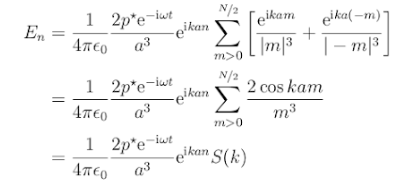
\includegraphics{Physics/trigon_exp.PNG}


Dosaíme li $E$ a tvar $p$ do pohybové rovnice dostaneme \ldots

$$
    \omega = \omega_0 \sqrt{ 1 - \frac{2}{a^3} k_e  \alpha S(k)}
$$

$$
    \omega_{k \to 0} = \omega_0 \left(  1  - k_e 2 \frac{\alpha}{a^3}  S(0)\right)
$$



    % \input{Physics/Einstein_Debeye_Heat_Capacity}

    % 
\subsection*{Ionizační energie elektronu vodíkového atomu}

\textbf{Určete ionizační energii elektronu pro základní stav vodíkového atomu a vyjádřete tuto energii v eV.}

\vspace{0.5cm}

Vyjdeme z Bohrova modelu atomu, který je postaven na postulátech:
\begin{enumerate}
    \item Elektron se může pohybovat po kruhových drahách (orbitech), takových, že 
    velikost momentu hybnosti elektronu $L = r p = r m_e v$ je celistvým násobkem $\bar h$ tj. $L_n = n \bar h = n\frac{h}{2\pi}$, kde $n = 1, 2, 3, \ldots$ je hlavní kvantové číslo.
    
    \small{Pro vlnovou délku platí de Broglieho vztah $\lambda = \frac{h}{p}$ a pro délku orbity $2\pi r = n \lambda = \frac{nh}{p} \therefore pr = n\hbar = L$}
    
    \item Elektron pohybující se po dovolených drahách nevyzařují energii.
    \item Elektron může přecházet pouze z jedno povolené orbity na jinou a při tomto přechodu vyzáří nebo pohltí příslušné množství energie o frekvenci $\nu  = \frac{E_f - E_i}{n}$. 
\end{enumerate}


Pro celkovou energii elektronu platí

\begin{equation}
    E = E_k + Ep = \frac{1}{2} m_e v^2 - \frac{e^2}{4\pi\epsilon_0 r^2}
\end{equation}

Kde druhý člen reprezentovaný Coulombovskou silou, představuje dostředivou sílu a tedy.

\begin{equation}\label{eq.2}
    \frac{e^2}{4\pi\epsilon_0 r^2} = m_e \frac{v^2}{r} \therefore m_e v^2 = \frac{e^2}{4\pi\epsilon_0 r}
\end{equation}

Dosadíme li do vzorce pro energii dostaneme:

\begin{equation}
    E = -\frac{e^2}{8\pi \epsilon_0 r}  =  -\frac{1}{2} m_e v^2
\end{equation}

Podle prvního postulátu o kvantování momentu hybnosti je $v = \frac{n\bar h}{m_e r}$ a tedy dosazením za rychlost a úpravou \ref{eq.2} získáme poloměr 

\begin{equation}
r_n = \frac{4\pi \hbar^2 \epsilon_0}{e^2 m_e} n^2
\end{equation} 

$r_1 \equiv a_0 \approx 0.53 A$ je tzv. Bohrův poloměr. Kvantování momentu hybnosti tedy způsobuje i kvantování poloměru orbitu. Tento poloměr opět můžeme dosadit do vzorce o energii a dostaneme

$$
    E_n = -\frac{e^4 m_e}{32\pi^2 \hbar^2 \epsilon_0^2} \frac{1}{n^2}
$$
a pro $n = 1$ je $r1$ poloměr základního stavu elektronu vodíkového atomu, kdy je elektron nejtěsněji vázán k jádru.

\begin{equation}
    E_1 = -\frac{e^4 m_e}{32\pi^2 \hbar^2 e_0^2} = 2.17 . 10^{-18} J = 13.6 eV.
\end{equation}

kde $1J = 6.241509⋅1018 eV$ a Rydbergova konstanta $Ry = \frac{e^2 m_e}{2\hbar^2}$.

\vspace{0.5cm}

Ionizační energie vodíkového atomu je energie potřebná k přemístění elektronu ze základního stavu do vzdálenosti $r \to \infty$ a je tedy rovna energii základního stavu $13.6 eV$.






    % % Continuum Mechanics

    % \part{MATEMATICKÉ MODELY}
    
    % These are study notes written along the course \textit{Language of Continuum Mechanics for Applied Geology} and \textit{Introduction to Mechanics of Fluids and Mixtures}

    % % - Fluid Mechanics
    % % - Solid Mechanics
    %     % \input{topic1-stress.tex}
    %     % \input{topic2-strain.tex}
    % 
\chapter{Modely popsané pomocí ODE} 

Typická obyčejná difrenciální rovnice prvního řádu

\begin{equation}
    u'(x) = -u(t), \quad x, t \in \R, \quad u: \R \mapsto \R,
\end{equation}
 doplněná počáteční podmínkou
 \begin{equation}
    u(0) = u_0, \quad u_0 \in \R,
 \end{equation}
jejímž řešením je funkce \footnote{Pro základní informace o řešení  obyčejných diferenciální rovnic lze nahlédnoud do Boyce a DiPrima nebo Braun.}
$$    
u(t) = u_0 \e{-t}.
$$

\noindent Řešení ověříme dosazením 

$$
u(0) = u_0 \e{0} = u_0
$$

$$
u'(t) = -u_0 \e{-t} = 
$$


\chapter{Modely popsané pomocí PDE}

\section{Značení}

Nechť $u := u(\vb{x}) $ je funkce $n$ proměnných tj. $\vb{x} \in \R^2$, $\vb{x} = (x_1,\ldots,x_3)$, potom pro parciální derivace použijeme značení 

$$
    \pdv{u}{x_1}, \quad \pdv{u}{x_1}{x_2}
$$
nebo 
$$
    u_{x_1}, \quad u_{x_1 x_2}
$$
nebo 
$$
    D^{\alpha}u,
$$
kde $D$ značí operátor.

\noindent Obecný polynom m-tého stupně:
$$
P(x) = \sum c_{\alpha} x^{\alpha}
$$

\noindent Binomická věta

\noindent Multinomická věta

\section{Diferenciální operátory}

Operátor \textbf{gradient} skalárního pole
$$
\grad{U} \equiv grad(U)
$$
operátor \textbf{divergence} (zřídlovost) vektorového pole
$$
\div{\vb V} \equiv div( \vb V)
$$
Operátor \textbf{rotace} (výřivost) vektorového pole
$$
\curl{\vb V} \equiv curl(\vb V)
$$
Laplacův operátor
$$
    \laplacian \equiv \Delta
$$

\section{Parciální diferenciální rovnice}

Parciální diferenciální rovnice je ve tvaru 

\begin{definition}[Parciální diferenciální rovnice]
$$
F = 0, \quad x \in \Omega \in \R^n
$$
je parciální diferenciální rovnice m-tého řádu, kde $F$ je skalární funkce a $u : \Omega \rightarrow{\R}$ je neznámá (hledaná) funkce.
\end{definition}

PDR je lineární pokud ji lze zapsat ve tvaru 
$$
$$
Pokud koeficienty $a_{\alpha}$ jsou konstantní tj. nezávisejí na $x$, jedná se o PDR s konstantními koeficienty.


PDR je semilineární (lineární vzhledem k nejvyšším derivacím)

PDR je kvazilineární

PDR je plně nelineární

\subsection{Otázky}
\begin{itemize}
    \item U tepelné nebo rovinné rovnice se někdy uvádí na pravé straně konstanta $k^2$ namísto $k$. Proč je tomu tak? 
\end{itemize}

\section{Úvod}

Řádem rovnice rozumíme řád nejvyšší derivace $u$ v rovnici.

\section{Typologie PDE}

\subsection{Rovnice eliptického typu}
\subsection{Rovnice parabolického typu}
Rovnice jako vedení tepla nebo difuze jsou označovaný jako rovnice parabolického tyypu.
\subsection{Rovnice hyperbolického typu}

Mnoho modelů popisujících difůzní proces má tu vlastnost, že po dostatečně dlouhém čase systém dosáhne ustáleného stavu. Jinak řečeno funkce $u(x, t)$ popisující stav systému se již němění s časem $t$, ale je pouze funkcí polohy $x$ $$ \therefore \partial_t u(x, t) = 0.$$ Pro tento ustálený neboli stacionární stav jsme schopni často nalézt stacionární (\textit{steady})i když neznáme obecné řešení zadané rovnice.   


\subsubsection{Příklad}
% \begin{enumarate}
%     \item  Tepelná energie se šíří vždy z místa s větší teplotou na místa s měnší teplotou.
% \end{enumerate}
% Mám laminární tok nestalčitelné substance a v něm umístěnou nekonečné malou krychlyčku o stranách $dx$, $dy$, $dz$. Potom 

Mějme parciální diferenciální rovnici s neznámou funkcí $u$ 

\begin{equation}
    \partial_t u = -\kappa \partial_{xx} u, \quad 0 < x < L, 0 < t <  \infty
\end{equation}
kde $u \equiv u(x, t)$ je funkcí místa $x$ a času $t \ge 0$ a $c > 0$ je konstanta. Na levé straně rovnice stojí derivace funkce $u$ vzhledem k času $t$ a vpravo její druhá derivace vzhldem k pozici $x$. Pro začátek ukážeme, že tato rovnice modeluje stacionární vedení tepla v tenkém drátu. 

Rovnice se také často udáva v homogenním tvaru, kdy všechny členy převedeme na jednu stranu.

\begin{equation}
    \partial_t u + \kappa \partial_{xx} u    = 0,
\end{equation}

\section{Ustálené vedení tepla bez zdroje}

\subsection{Formulace pro 1D}
Předpokládejme, že rovný drát konéčné délky $L$ leží podél intervalu $[0, L]$ na ose $x$. Také předpokládejme, že je z homogenního materiálů a stejné hustotě a tedy, že má v celé délce stejné vlastnosti a také, že jeho teplota nemá na tyto vlastnosti vliv. To znamená, že schopnost vést teplo ani délka se s teplotou nemění. \footnote{ Vlastnosti materiálu, jako objem a schopnost vést teplo aj., jsou obvykle závislé na teplotě.}

\subsection{Formulace pro 2D}

\section{Ustálené vedení tepla se zdrojem}

\subsection{Formulace pro 1D}
\subsection{Formulace pro 2D}

\section{Neustálené vedení tepla s anizotropií}

% Rovnice vedení tepla v přímém \footnote{Pokud drát nebyl přímý, má to vliv na úlohu?} drátu o délce $l$, můžeme při zanedbání jeho průměru, považovat za problém v jedné prostorové dimenzi, kdy nás zajímá průběh teploty drátu v jeho libovolném místě $x$ a v čase $t$. Rovnice vedení tepla v diferenciální formě má pak podobu  

% Problém řešení rovnice vedení tepla v tyči o konstaním průřezu a délce můžeme zjednodušit na problém v jedné dimenzi, pokud jdenodudše dělíme tok plochou průřezu kolmou na směr šíření tepla.

% \begin{equation}
%     \frac{\partial u}{\partial t} = \lamda \frac{\partial \varphi}{\partial t}, 
% \end{equation}
% where $u = u(x, t)$ is temperature at point $x$ and time $t$. 

\section{Difuze}

\section{Šíření vlny aneb \textit{Wave Equation}} 

\begin{equation}
    \partial_{tt} u = -\kappa \partial_{xx} u,
\end{equation}
\begin{equation}
    \frac{\partial^2 u}{\partial t^2} = -\kappa \frac{\partial_{xx} u,
\end{equation}

\section{Rovnice mělké vody}

řešením parciálních diferenciálních rovnic popisujících proudění tzv. mělké vody, kde zanedbáváme toky ve svislém směru. Tyto rovnice jsou hyperbolického typu 1. řádu s reaktivním členem daným topologií dna.

Diplomové práce z MFF práce věnující se tomuto 

\begin{itemize}
    \item https://dspace.cuni.cz/handle/20.500.11956/85985
    \item https://dspace.cuni.cz/handle/20.500.11956/39804
    \item https://dspace.cuni.cz/handle/20.500.11956/84466
\end{itemize}
    
    % \part{NUMERICKÉ METODY}
    %     \input{num/num0}
\end{document}





